\chapter{Implementation of Remotely Tunable MT-FRHC based G-FLCS with VBCoA on Programmable DSP}

\begin{chapterAbstract}{Preview}
	This chapter present a MT-FRHC based remotely tunable G\hyp{}FLC implemented on a programmable DSP platform. The algorithm is ported on a single core fixed point DSP, which can be remotely configured in real\hyp{}time over Ethernet. This feature of reconfigurability enables a user to change fuzzy parameters in real\hyp{}time, eliminating repeated hardware programming. The scheme also eliminates the requirement of removing the controller from the process plant for configuration. A hardware software co\hyp{}design architecture for the proposed generic FLC is developed on TI C6748 DSP with Sys/BIOS RTOS and seamlessly integrated with a web based user interface (WebUI) for reconfigurability. The WebUI acquires the fuzzy parameters from users and a server application is dedicated to data communication between the hardware and the server. Analysis of this design is carried out by using hardware\hyp{}in\hyp{}loop (HIL) test to control various plant models in Simulink/Matlab environment. Performance of the proposed system is compared to Fuzzy Toolbox of Matlab and PID controllers.
\end{chapterAbstract}
\clearpage

\section{Introduction}
In previous chapter, the proposed MT-FRHC based remotely tunable G-FLCS architecture with Genetic Algorithm based FCP extraction technique is described. The results convincingly depicted that the objectives set in chapter 1 can be achieved in simulation environment. This chapter extrapolates the concepts introduced in last chapter to implementation it on a DSP platform. This chapter also introduces implementation and optimization of the code to realize the proposed MT-FRHC based G-FLCS with VBCoA defuzzification method. It is important that the code size is reduced to its maximum for reliable operation of the system. Large code size decreases power efficiency and computational speed. Smaller code size require less memory fetching since larger part of the on chip memory will be available for execution. This also increases the stack size. In this implementation it is imperative that the code size is limited to 60\% of the on-chip SHRAM.

\section{Hardware Device: TI LCDK C6748}
To achieve an efficient implementation, it is important to understand the architecture of th hardware device before final implementation. With a sequential processing on a DSP device, the objective of the proposed MT-FRHC based G-FLCS with VBCoA defuzzification to meet 11K FLIPS achieved by Yi Fu et. al. \cite{Fu2010} for their G-FLCS architecture on an FPGA is unachievable. Hereby, the implementation of the proposed G-FLCS architecture has to be parallelized. With this context, the hardware device at hand, TI's LCDK C6478 needs to be inspected.

LCDK C6478 incorporates a TMS320C6748 DSP which is a floating point very long instruction word (VLIW) DSP processor running at 476 MHz clock frequency. This device supports SIMD (single instruction, multiple data)and double precision VLIW operations \cite{TexasInstruments2013}. It is reported that this is one of the speediest single precision device. This is an important feature of this device that suits the proposed G-FLCS architecture since all operations are single precision. SIMD instructions supports data parallelism as opposed to VLIW's instruction parallelism. To take leverage of the SIMD or VLIW operations, it is imperative that the typical architecture of the G-FLCS is reconsidered to match either of these features of the device considering the functional block diagram in \ref{fig:functional_block}. 

\begin{figure}[h]
\centering
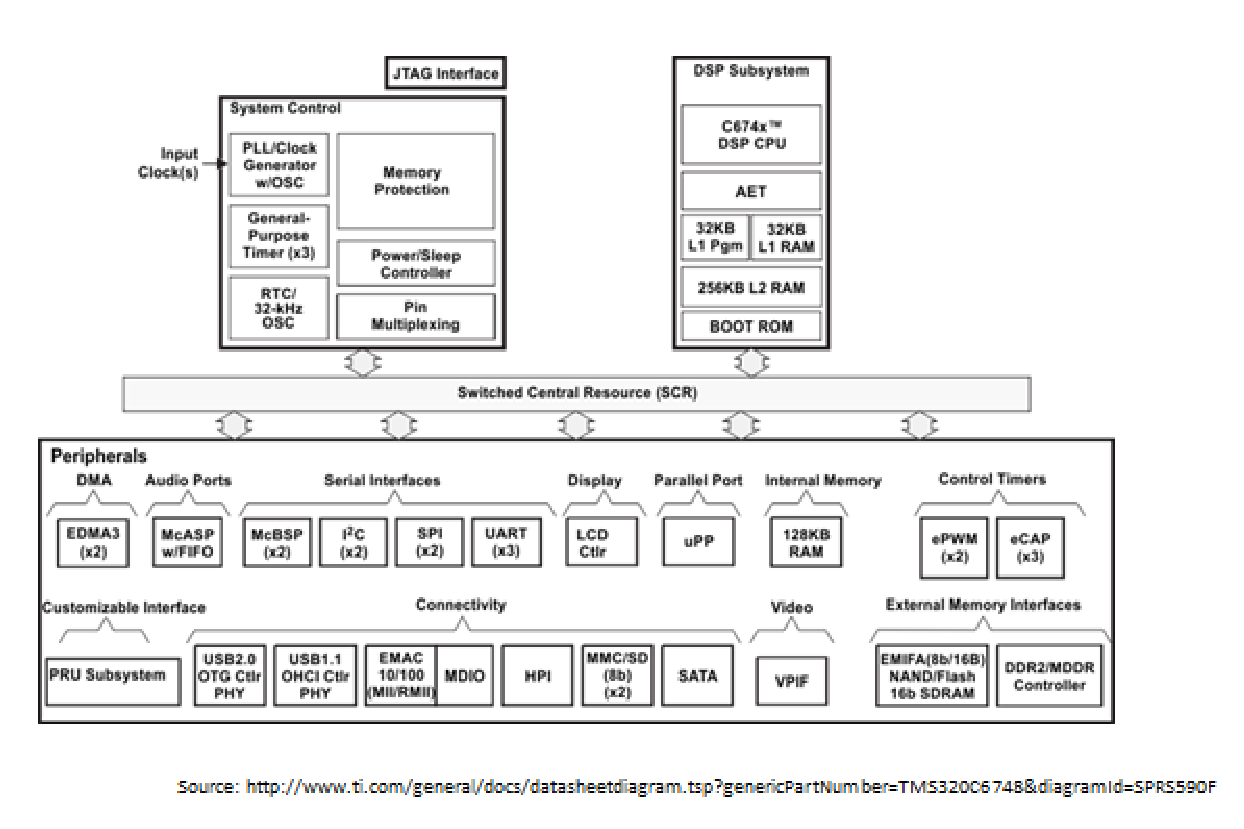
\includegraphics[width=0.9\linewidth]{Chapter4/chapter4/functional_block}
\caption{Functional Block Diagram of TMS320C6748 DSP}
\label{fig:functional_block}
\end{figure}

\section{Generic FLC on DSP (TI LCDK C6748)}
\subsection{System Architecture}
The system architecture of the proposed MT-FRHC based G-FLCS is represented as shown in \eqref{eq:MFRHC-final},
\begin{equation} 
{\theta _f}({c_j}) = \bigcap\limits_{{k_x} = 0}^{n_{op} - 1} {\left( {{\theta _f}\left( {{R_b}\left( {{k_x}} \right)} \right),\left( {\bigcup\limits_{l = 0}^{N - 1} {\overrightarrow {{C_{{R_v}}}\left( l \right)} } } \right)} \right)} 
\end{equation}
There are two data loops in this architecture. The inner loop is set to a small constant by the number of active MFs (in this case completely controlled by the user); while the outer loops are independent of the data. Therefore it can be concluded that the dependency of the outer loop is already parallelized in this architecture.

\subsection{Code Optimization} \label{sec:subsec1}
Generally a code that is written in assembly (ASM) is processor\hyp{}specific, whereas C code can readily be ported from one platform to another. However, optimized ASM code runs faster than C and requires less memory space. Before optimizing a code, it is required to make sure that the code is functional and yields correct results. After optimizing, the code can be reorganized and resequenced. The code becomes extremely difficult to follow and debug. It needs to be realized that if a C\hyp{}coded algorithm is functional and its execution speed is satisfactory, there may not be a necessity to optimize it further. All these motivates us to stretch the optimization so that the best possible efficiency is extracted from the system \cite{TexasInstruments2014,Batten2000}.
A rigorous code optimization strategy was devised as follows\cite{bookchassaing2005}:
\begin{description}
	\item[Step 1] G\hyp{}FLC is programmed in C Language without using any compiler optimization levels. With help of CCS Profiler tool, all the submodules are inspected for performance with respect to execution time and memory consumed.
	\item[Step 2] Intrinsic functions are used along with various compiler optimization levels. Functions like minimum (min), maximum (max), product (prod), division (div) are written as intrinsic functions and called as necessary by the modules and submodules of hardware G\hyp{}FLCS.
	\item[Step 3] Thereafter, the CCS Profiler tool is exploited again to determine and identify the functions and submodules that may need further optimization. 
	\item[Step 4] The functions that do not meet expected time and memory budget, are converted to linear ASM. The resultant is again inspected using the CCS Profiler tool to check for final efficiency.
\end{description}

 These process is realized in the system as follows: 
 \begin{enumerate}
 	\item `-o3' with optimization `-mt' 
 	\item `-k' with optimization `-mw' as feedback option for compiler
 	\item Minimize the loop carried dependency bound. 
 	\item MUST\_ITERATE and UNROLL pragmas.
 	\item Operate on single precision data type
 	\item SIMD
 	\item Intrinsics from TI library.
 \end{enumerate}

 \begin{table}[h]
 	\centering
 	\caption{Options in Compiler Level Optimization}
 	\label{tab:opti_param}
 	\resizebox{0.85\textwidth}{!}{%
 		\begin{tabular}{cc}
 			\hline
 			Options & Features \\ \hline
 			-o3 & \begin{tabular}[c]{@{}c@{}}This activates Compiler optimization level 3. \\ In this setting, the compiler majorly tries to \\ perform software pipelining.It also converts \\ small functions to inline calls.\end{tabular} \\ \hline
 			-mt & \begin{tabular}[c]{@{}c@{}}It explicitly mentions that the pointer-based \\ parameters of a function will never point to \\ the same location.\end{tabular} \\ \hline
 			-k, -mw & \begin{tabular}[c]{@{}c@{}}These options instruct the compiler to \\ generate feedback which can be analyzed \\ for tuning performance.\end{tabular} \\ \hline
 		\end{tabular}%
 	}
\end{table}

The compiler can insert calls to special functions in the run\hyp{}time support library (RTS) to support operations that are not natively supported by the ISA. For example, the compiler calls $\_\_c6xabi\_divi() $ ($ \_divi() $ in COFF) function to perform 32\hyp{}bit integer divide operation. Such functions are called compiler helper functions, and result in a function call within the loop body. For example in G\hyp{}FLC, the compiler accomplishes the division operation by calling the compiler helper function "$ \_divi $" in fuzzification and defuzzification modules.

\subsection{Code Implementation}
\begin{figure}[h!]
	\centering
	\subfloat[Without Optimization]{\label{fig:fig4_1}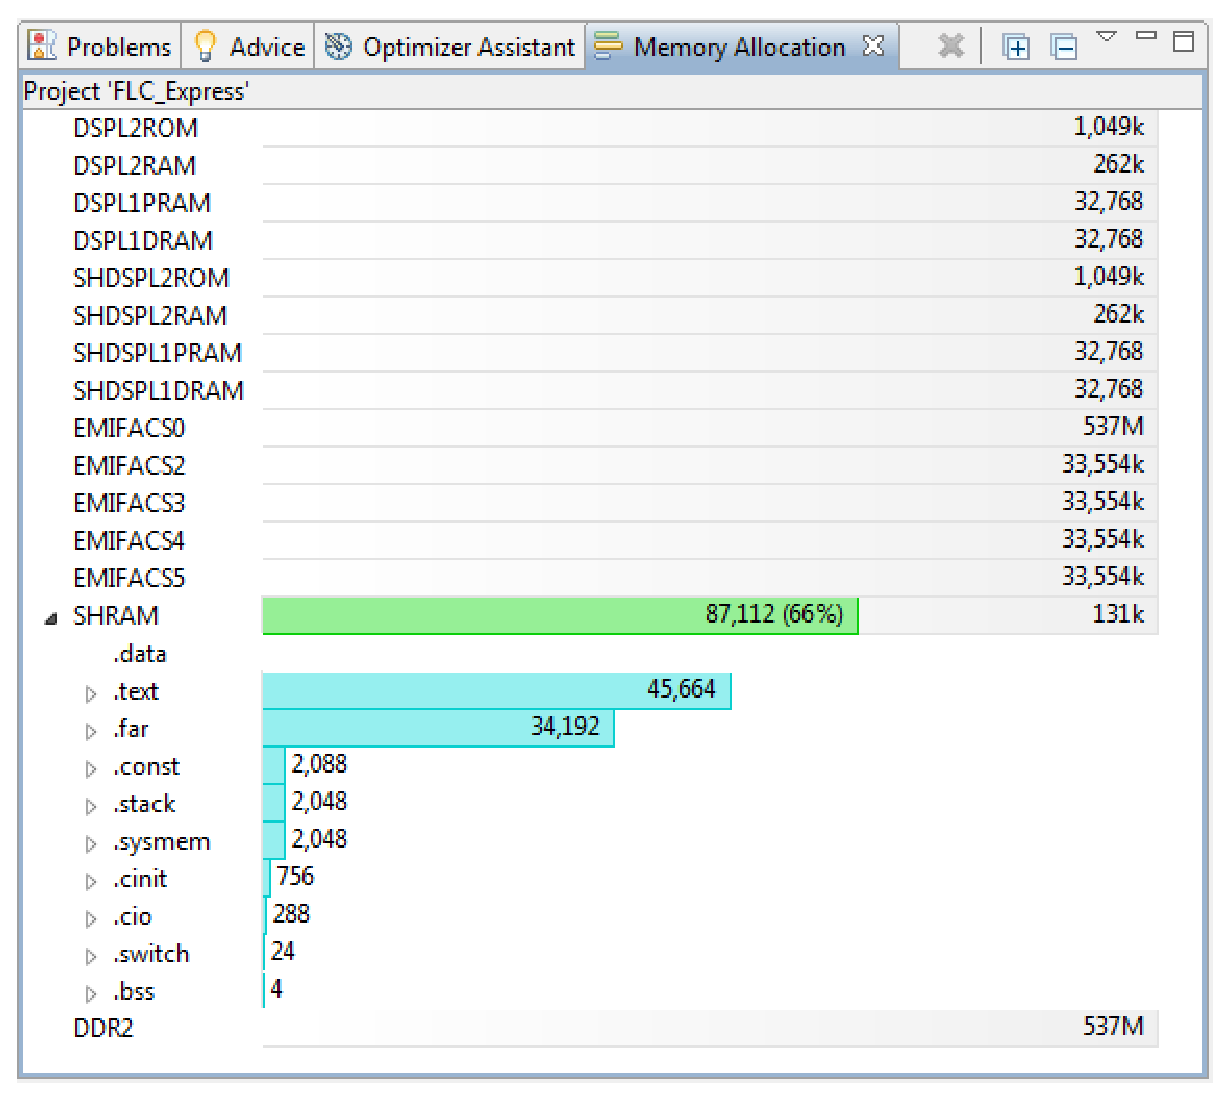
\includegraphics[width=0.95\linewidth,height=0.4\textheight]{Chapter4/chapter4/Fig1_MU}} \\
	\subfloat[Optimization]{\label{fig:fig4_2}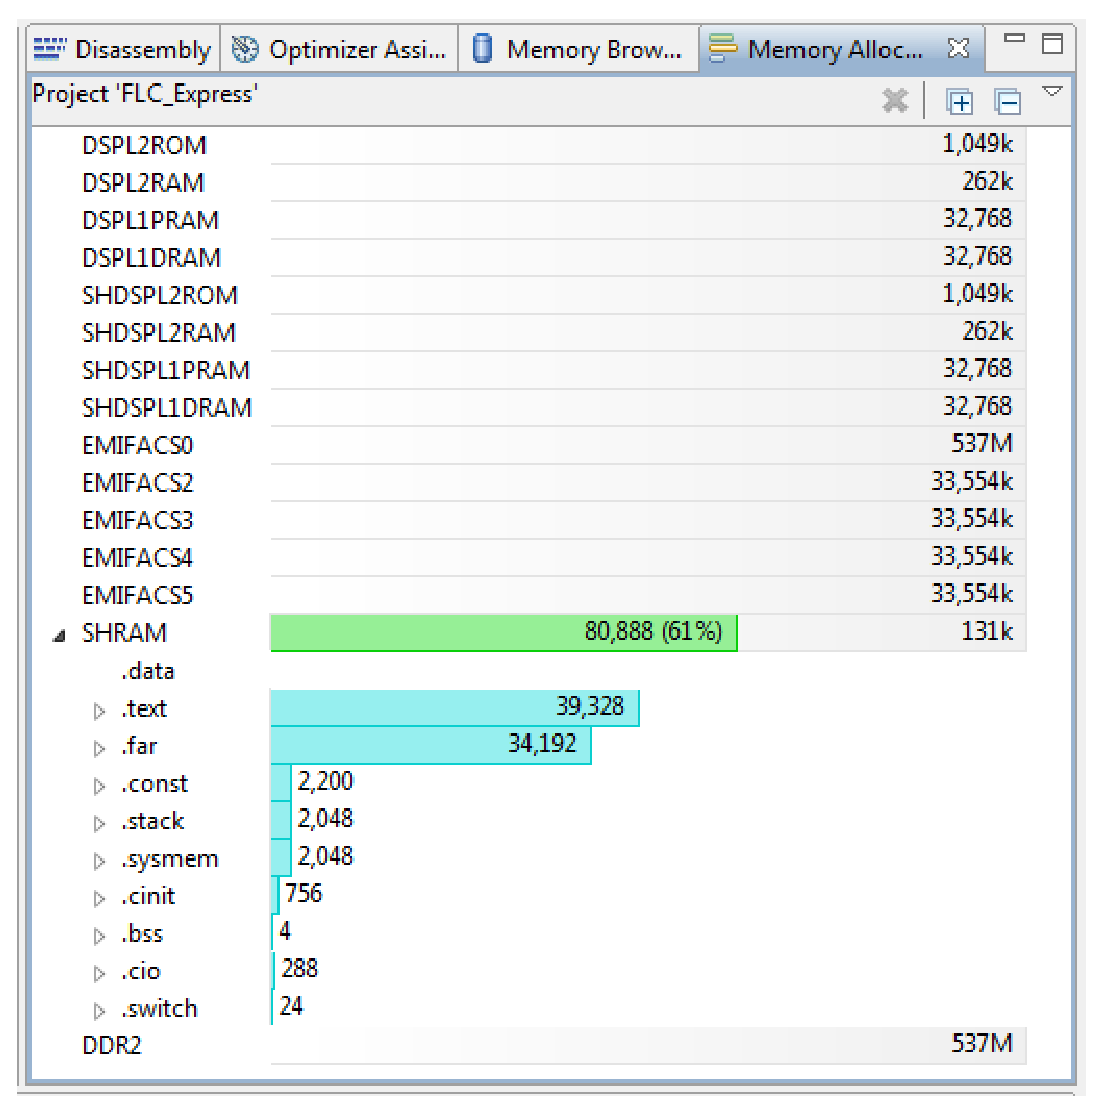
\includegraphics[width=0.95\linewidth,height=0.4\textheight]{Chapter4/chapter4/Fig2_MU_Opti}} 
	\caption{Memory Utilization of Proposed System Realized on TI C6748 DSP}
	\label{fig:Mem_Util}
\end{figure}
Code Composer Studio (CCS) is a proprietary integrated development environment developed by TI for programming DSP and ARM processors. The design is programmed in C language and optimized as described in section \ref{sec:subsec1}. Thereafter it is cross compiled using CCS v5.5 compiler and implemented on TMS320C6748 as target DSP processor. This system represents the hardware G\hyp{}FLCS as discussed previously. G\hyp{}FLCS is connected to a server PC using on\hyp{}board UART and provides a platform which is capable of accepting FCP file to operate as a standalone tunable G\hyp{}FLCS.

To achieve a high performance in throughput, the following optimization technique were used inside the developed code \cite{TexasInstruments2013}.
\begin{description}
	\item[The MUST\_ITERATE Pragma] The MUST\_ITERATE pragma specifies the lower bound, upper bound and factors of a loop. The lower bound and upper bound specifically mentions the minimum and maximum possible iterations of the loop and the factor defines the step size between them.
	\begin{lstlisting}[language=C,caption={MUSTITERATE Pragma},label=CS:constraints]
		#pragma MUST_ITERATE(lower_bound, upper_bound, factor)
	\end{lstlisting}
	\item[Loop Unrolling and the UNROLL Pragma] Manual unroll of loops are imbibed in code to improve code efficiency. Consider following code snippets.
	\begin{lstlisting}[language=C,caption={A Loop Code With Unbalanced Resource Partition},label=CS:constraints]	
	void Loop(int * restrict output, int * restrict input1, int * restrict input2, int n)
	{
	int i;
	for (i=0; i<n; i++)
	{
	output[i] = input1[i] + input2[i];
	}
	}
	//An excerpt from its compiler feedback
	;* Partitioned Resource Bound(*) : 2
	;* Resource Partition:
	;* A-side B-side
	;* .L units 0 0
	;* .S units 0 1
	;* .D units 2* 1
	;* .M units 0 0
	\end{lstlisting}
	The .D unit on the A side of the device is used twice every iteration, and the .D unit on the B side is only used once. This indicates that the .D unit on the B side is left open for 1 cycle in each iteration of the loop. In this case, the partitioned resource bound is affected by this unbalanced partition. Ideally, it would be more efficient if both units are used 1.5 cycles per iteration or 3 cycles per 2 iterations
	\begin{lstlisting}[language=C,caption={Manually Unrolled Loop},label=CS:constraints]
	void Loop(int * restrict output, int * restrict input1, int * restrict input2, int n)
	{
	int i;
	for (i=0; i<n; i+=2)
	{
	output[i] = input1[i] + input2[i];
	output[i+1] = input1[i+1] + input2[i+1];
	}
	}
	//An excerpt from its compiler feedback
	;* Partitioned Resource Bound(*) : 3
	;* Resource Partition:
	;* A-side B-side
	;* .L units 0 0
	;* .S units 1 0
	;* .D units 3* 3*
	;* .M units 0 0		
	\end{lstlisting}
	The .D units are used 3 times on each side per iteration, but the number of iterations is halved. This, in theory, can lead to a 25\% reduction in overall cycle count. Although effective, the manual unroll process can be tedious for most loops. Generally, it is recommended that the C6000 compiler and pragmas be used to unroll loops.
\end{description}

Detailed memory utilization of the built code is shown in Figure \ref{fig:Mem_Util}. It can be observed that the code size without optimization acquires 66\% of the SHRAM and has a code size of 88K. After employing the optimization strategy, the code size is reduced to 61\% of the SHRAM with a code size of 80K.

\section{Interfacing G\hyp{}FLC with WebUI}
\subsection{Data Communication between Hardware G\hyp{}FLCS and Server}
The proposed system architecture involves hardware\hyp{}software co\hyp{}design to present a complete reconfigurable FLC. The WebUI in client server model represents the software and the driver layer to interface the hardware G\hyp{}FLCS through serial port as shown in Figure \ref{fig:ProposedFLCArchitecturalDesign}. The DSP hardware receives FCP data serially and stores them in predefined memory locations as shown in Table \ref{tab:memorymap}. These parameters which are, segregated in two categories namely \textit{Setup} and \textit{Rulebase} data. The driver layer in the hardware G\hyp{}FLCS receives and acknowledges the data transmission serially over UART. 

%Elaborate about the serial communication and other communication protocols like CAN, Modbus, Profibus etc.

\begin{table}[h!]
	\centering
	\caption{Memory Map}
	%		\tiny
	\resizebox{0.9\textwidth}{!}{\begin{tabular}{@{}llll@{}}
			\toprule
			\multicolumn{1}{c}{\textbf{Offset Addr.}} & \multicolumn{1}{c}{\textbf{Memory bits}} & \multicolumn{1}{c}{\textbf{Description}} & \multicolumn{1}{c}{\textbf{Details}} \\ \midrule
			\multicolumn{1}{|l|}{\multirow{4}{*}{00H}} & \multicolumn{1}{l|}{\multirow{4}{*}{{[}1:0{]}}} & \multicolumn{1}{l|}{00-No Operation} & \multicolumn{1}{l|}{\multirow{4}{*}{\begin{tabular}[c]{@{}l@{}}To start the FLC operation for the \\ first time programmed with 0x03h \\ then if input only changes program \\ with 0x01H\end{tabular}}} \\
			\multicolumn{1}{|l|}{} & \multicolumn{1}{l|}{} & \multicolumn{1}{l|}{01-New inputs are enables} & \multicolumn{1}{l|}{} \\
			\multicolumn{1}{|l|}{} & \multicolumn{1}{l|}{} & \multicolumn{1}{l|}{10-new Rulebase is enabled} & \multicolumn{1}{l|}{} \\
			\multicolumn{1}{|l|}{} & \multicolumn{1}{l|}{} & \multicolumn{1}{l|}{11- new Rulebase and inputs are enabled} & \multicolumn{1}{l|}{} \\ \midrule
			\multicolumn{1}{|l|}{00H} & \multicolumn{1}{l|}{{[}7:2{]}} & \multicolumn{1}{l|}{\textbf{Don't Care}} & \multicolumn{1}{l|}{} \\ \midrule
			\multicolumn{1}{|l|}{\multirow{4}{*}{01H}} & \multicolumn{1}{l|}{\multirow{4}{*}{{[}1:0{]}}} & \multicolumn{1}{l|}{00- Number of inputs = 1} & \multicolumn{1}{l|}{\multirow{6}{*}{Number of Inputs and Outputs}} \\
			\multicolumn{1}{|l|}{} & \multicolumn{1}{l|}{} & \multicolumn{1}{l|}{01- Number of inputs = 2} & \multicolumn{1}{l|}{} \\
			\multicolumn{1}{|l|}{} & \multicolumn{1}{l|}{} & \multicolumn{1}{l|}{10- Number of inputs = 3} & \multicolumn{1}{l|}{} \\
			\multicolumn{1}{|l|}{} & \multicolumn{1}{l|}{} & \multicolumn{1}{l|}{11- Number of inputs = 4} & \multicolumn{1}{l|}{} \\ \cmidrule(r){1-2}
			\multicolumn{1}{|l|}{\multirow{2}{*}{01H}} & \multicolumn{1}{l|}{\multirow{2}{*}{{[}2{]}}} & \multicolumn{1}{l|}{0- Number of outputs = 1} & \multicolumn{1}{l|}{} \\
			\multicolumn{1}{|l|}{} & \multicolumn{1}{l|}{} & \multicolumn{1}{l|}{1- Number of outputs = 2} & \multicolumn{1}{l|}{} \\ \midrule
			\multicolumn{1}{|l|}{01H} & \multicolumn{1}{l|}{{[}7:3{]}} & \multicolumn{1}{l|}{\textbf{Don't Care}} & \multicolumn{1}{l|}{} \\ \midrule
			\multicolumn{1}{|l|}{02H} & \multicolumn{1}{l|}{{[}2:0{]}} & \multicolumn{1}{l|}{Number of MFs for Input 1} & \multicolumn{1}{l|}{\multirow{6}{*}{\begin{tabular}[c]{@{}l@{}}000- 0 (I/O not used),\\ 001- 111 refers to the number 1-7\end{tabular}}} \\ \cmidrule(r){1-2}
			\multicolumn{1}{|l|}{02H} & \multicolumn{1}{l|}{{[}4:6{]}} & \multicolumn{1}{l|}{Number of MFs for Input 2} & \multicolumn{1}{l|}{} \\ \cmidrule(r){1-2}
			\multicolumn{1}{|l|}{03H} & \multicolumn{1}{l|}{{[}2:0{]}} & \multicolumn{1}{l|}{Number of MFs for Input 3} & \multicolumn{1}{l|}{} \\ \cmidrule(r){1-2}
			\multicolumn{1}{|l|}{03H} & \multicolumn{1}{l|}{{[}6:4{]}} & \multicolumn{1}{l|}{Number of MFs for Input 4} & \multicolumn{1}{l|}{} \\ \cmidrule(r){1-2}
			\multicolumn{1}{|l|}{04H} & \multicolumn{1}{l|}{{[}2:0{]}} & \multicolumn{1}{l|}{Number of MFs for Output 1} & \multicolumn{1}{l|}{} \\ \cmidrule(r){1-2}
			\multicolumn{1}{|l|}{04H} & \multicolumn{1}{l|}{{[}6:4{]}} & \multicolumn{1}{l|}{Number of MFs for Output 2} & \multicolumn{1}{l|}{} \\ \midrule
			\multicolumn{4}{|l|}{\textit{\begin{tabular}[c]{@{}l@{}}MFs consists of type of MF and the number of co-ordinates are based on them. \\ Each input and output can have maximum of 7 MFs.\end{tabular}}} \\ \midrule
			\multicolumn{4}{|l|}{\textbf{MFs for Input 1}} \\ \midrule
			\multicolumn{1}{|l|}{05H} & \multicolumn{1}{l|}{{[}7:0{]}} & \multicolumn{1}{l|}{1st Co-ordinate of MF 1 of input 1} & \multicolumn{1}{l|}{\multirow{4}{*}{MF 1 of Input 1}} \\ \cmidrule(r){1-2}
			\multicolumn{1}{|l|}{06H} & \multicolumn{1}{l|}{{[}7:0{]}} & \multicolumn{1}{l|}{2nd Co-ordinate of MF 1 of input 1} & \multicolumn{1}{l|}{} \\ \cmidrule(r){1-2}
			\multicolumn{1}{|l|}{07H} & \multicolumn{1}{l|}{{[}7:0{]}} & \multicolumn{1}{l|}{3rd Co-ordinate of MF 1 of input 1} & \multicolumn{1}{l|}{} \\ \cmidrule(r){1-2}
			\multicolumn{1}{|l|}{08H} & \multicolumn{1}{l|}{{[}7:0{]}} & \multicolumn{1}{l|}{4th Co-ordinate of MF 1 of input 1} & \multicolumn{1}{l|}{} \\ \midrule
			\multicolumn{1}{|l|}{\multirow{5}{*}{09H}} & \multicolumn{1}{l|}{\multirow{5}{*}{{[}2:0{]}}} & \multicolumn{1}{l|}{\multirow{5}{*}{Type of MF number 1 of input 1}} & \multicolumn{1}{l|}{000- Trapezoidal} \\ \cmidrule(l){4-4} 
			\multicolumn{1}{|l|}{} & \multicolumn{1}{l|}{} & \multicolumn{1}{l|}{} & \multicolumn{1}{l|}{001- Gbell} \\ \cmidrule(l){4-4} 
			\multicolumn{1}{|l|}{} & \multicolumn{1}{l|}{} & \multicolumn{1}{l|}{} & \multicolumn{1}{l|}{010- Gaussian} \\ \cmidrule(l){4-4} 
			\multicolumn{1}{|l|}{} & \multicolumn{1}{l|}{} & \multicolumn{1}{l|}{} & \multicolumn{1}{l|}{011- Curved Triangle} \\ \cmidrule(l){4-4} 
			\multicolumn{1}{|l|}{} & \multicolumn{1}{l|}{} & \multicolumn{1}{l|}{} & \multicolumn{1}{l|}{100- 111- Triangle} \\ \midrule
			\multicolumn{1}{|l|}{...} & \multicolumn{1}{l|}{...} & \multicolumn{1}{l|}{...} & \multicolumn{1}{l|}{MF 2-7, Input 1} \\ \midrule
			\multicolumn{4}{|l|}{\textbf{MFs for Input 2}} \\ \midrule
			\multicolumn{1}{|l|}{28H} & \multicolumn{1}{l|}{{[}7:0{]}} & \multicolumn{1}{l|}{1st Co-ordinate of MF 1 of input 2} & \multicolumn{1}{l|}{\multirow{4}{*}{MF 1 Input 2}} \\ \cmidrule(r){1-3}
			\multicolumn{1}{|l|}{3AH} & \multicolumn{1}{l|}{{[}7:0{]}} & \multicolumn{1}{l|}{2nd Co-ordinate of MF 1 of input 2} & \multicolumn{1}{l|}{} \\ \cmidrule(r){1-3}
			\multicolumn{1}{|l|}{3BH} & \multicolumn{1}{l|}{{[}7:0{]}} & \multicolumn{1}{l|}{3rd Co-ordinate of MF 1 of input 2} & \multicolumn{1}{l|}{} \\ \cmidrule(r){1-3}
			\multicolumn{1}{|l|}{3CH} & \multicolumn{1}{l|}{{[}7:0{]}} & \multicolumn{1}{l|}{4th Co-ordinate of MF 1 of input 2} & \multicolumn{1}{l|}{} \\ \midrule
			\multicolumn{1}{|l|}{3DH} & \multicolumn{1}{l|}{{[}2:0{]}} & \multicolumn{1}{l|}{Type of MF number 1 of input 2} & \multicolumn{1}{l|}{000- 111 (Same as above)} \\ \midrule
			\multicolumn{1}{|l|}{...} & \multicolumn{1}{l|}{...} & \multicolumn{1}{l|}{...} & \multicolumn{1}{l|}{} \\ \midrule
			\multicolumn{1}{|l|}{D6H} & \multicolumn{1}{l|}{{[}2:0{]}} & \multicolumn{1}{l|}{Type of MF number 7 of output 2} & \multicolumn{1}{l|}{} \\ \midrule
			\multicolumn{4}{|l|}{\textit{Memory is reserved for 4 Inputs and 2 Outputs consequently even if, FLC does not operate with all 4 input and 2 output.}} \\ \midrule
			\multicolumn{4}{|l|}{\textbf{Rule 1}} \\ \midrule
			\multicolumn{1}{|l|}{D7H} & \multicolumn{1}{l|}{{[}3:0{]}} & \multicolumn{1}{l|}{Index number of Input 1} & \multicolumn{1}{l|}{\multirow{6}{*}{\begin{tabular}[c]{@{}l@{}}000- 0 (I/O not used),\\ 001- 111 refers to the number 1-7\end{tabular}}} \\ \cmidrule(r){1-3}
			\multicolumn{1}{|l|}{D7H} & \multicolumn{1}{l|}{{[}7:4{]}} & \multicolumn{1}{l|}{Index number of Input 2} & \multicolumn{1}{l|}{} \\ \cmidrule(r){1-3}
			\multicolumn{1}{|l|}{D8H} & \multicolumn{1}{l|}{{[}3:0{]}} & \multicolumn{1}{l|}{Index number of Input 3} & \multicolumn{1}{l|}{} \\ \cmidrule(r){1-3}
			\multicolumn{1}{|l|}{D8H} & \multicolumn{1}{l|}{{[}7:4{]}} & \multicolumn{1}{l|}{Index number of Input 4} & \multicolumn{1}{l|}{} \\ \cmidrule(r){1-3}
			\multicolumn{1}{|l|}{D9H} & \multicolumn{1}{l|}{{[}3:0{]}} & \multicolumn{1}{l|}{Index number of Output 1} & \multicolumn{1}{l|}{} \\ \cmidrule(r){1-3}
			\multicolumn{1}{|l|}{D9H} & \multicolumn{1}{l|}{{[}7:4{]}} & \multicolumn{1}{l|}{Index number of Output 2} & \multicolumn{1}{l|}{} \\ \midrule
			\multicolumn{4}{|l|}{\textbf{Rule 2}} \\ \midrule
			\multicolumn{1}{|l|}{...} & \multicolumn{1}{l|}{...} & \multicolumn{1}{l|}{...} & \multicolumn{1}{l|}{} \\ \midrule
			\multicolumn{4}{l}{\textit{\textbf{Continues till end of rules. Max rules supported by this system is 2401 (7\textasciicircum 4)}}} \\ \bottomrule
		\end{tabular}
	}
	\label{tab:memorymap}
\end{table}

\subsection{WebUI and its Operation}
The WebUI is a web application that drives the proposed hardware G\hyp{}FLCS was presented in section \ref{sec:WebUI} and displayed in Figure \ref{fig:WebUI} and Figure \ref{fig:WebUI2} stores FCP data in a file\footnote{File can be downloaded from \url{https://goo.gl/YAVxez}}. It may be noted that the FCP file is generated deliberately in accordance with Matlab Fuzzy Inference System (FIS) file format to provide liberty to integrate a parameter data file generated using Matlab Fuzzy Logic Toolbox as well. Submitting the parameters triggers a desktop application that is native to the server. Objective of this program is to transmits the FCP from database to the hardware G\hyp{}FLCS through serial communication. The FCP data is stored in the DSP board based according to the memory map provided in Table \ref{tab:memorymap}. The first column in Table \ref{tab:memorymap} shows the offset address and the second column elaborates the number of bit individual fuzzy parameter consumes. The last two columns describes and provides remarks about the different fuzzy parameters FLC designed with M\hyp{}FRHC rule reducing Inference Engine, operates on the inputs with these FCP data to provide desired control action. FCP data is segregated in two parts, \textit{Setup} and \textit{Rulebase}. Offset address \textbf{0000}H to \textbf{00D6}H in Table \ref{tab:memorymap} shows the details of Setup parameters. \textit{Rulebase} parameters appear in memory location \textbf{00D7}H to \textbf{1D0C}H which is reserved to store \textbf{{2401}} ~rules. Fuzzifier, inference engine and defuzzifier is programmed with information about the data and its memory location. With these information, fuzzifier transforms crisp inputs in fuzzy domain and a Mamdani inference engine, coupled with the Rulebase in the system memory produces fuzzy output. Defuzzifier transforms fuzzy output compiled by the inference engine back to crisp output.

The Memory Map in Table \ref{tab:memorymap} is also segregated into two parts as FCP data. The first part, incorporates the \textit{Setup} FCP data, specifies the Fuzzifier and Defuzzifier parameters and it includes the following information;
\begin{itemize}
	\item Initialization of the FLC,
	\item Number of Inputs and Outputs,
	\item Number of Membership Functions in each Input and Output, and
	\item Details of each Membership Functions like, type of membership function and their co-ordinates.
\end{itemize}

The second part, incorporates \textit{Rulebase} FCP data, specifies the Rulebase of the FLC defined by the index numbers of the inputs and outputs.
In this work, the original user specified Fuzzy Control Parameters (FCP) (as specified in the Table \ref{tab:memorymap} Memory Map) is not forked or pruned. Rather, at every inference the proposed MT-FRHC rule reduction algorithm, operates on this user specified Memory Map to derive another map with reduced rules. 
 

\section{System Performance and Analysis}

\subsection{System Modeling of Armature Controlled DC Motor}
\begin{figure}[h!]
	\centering
	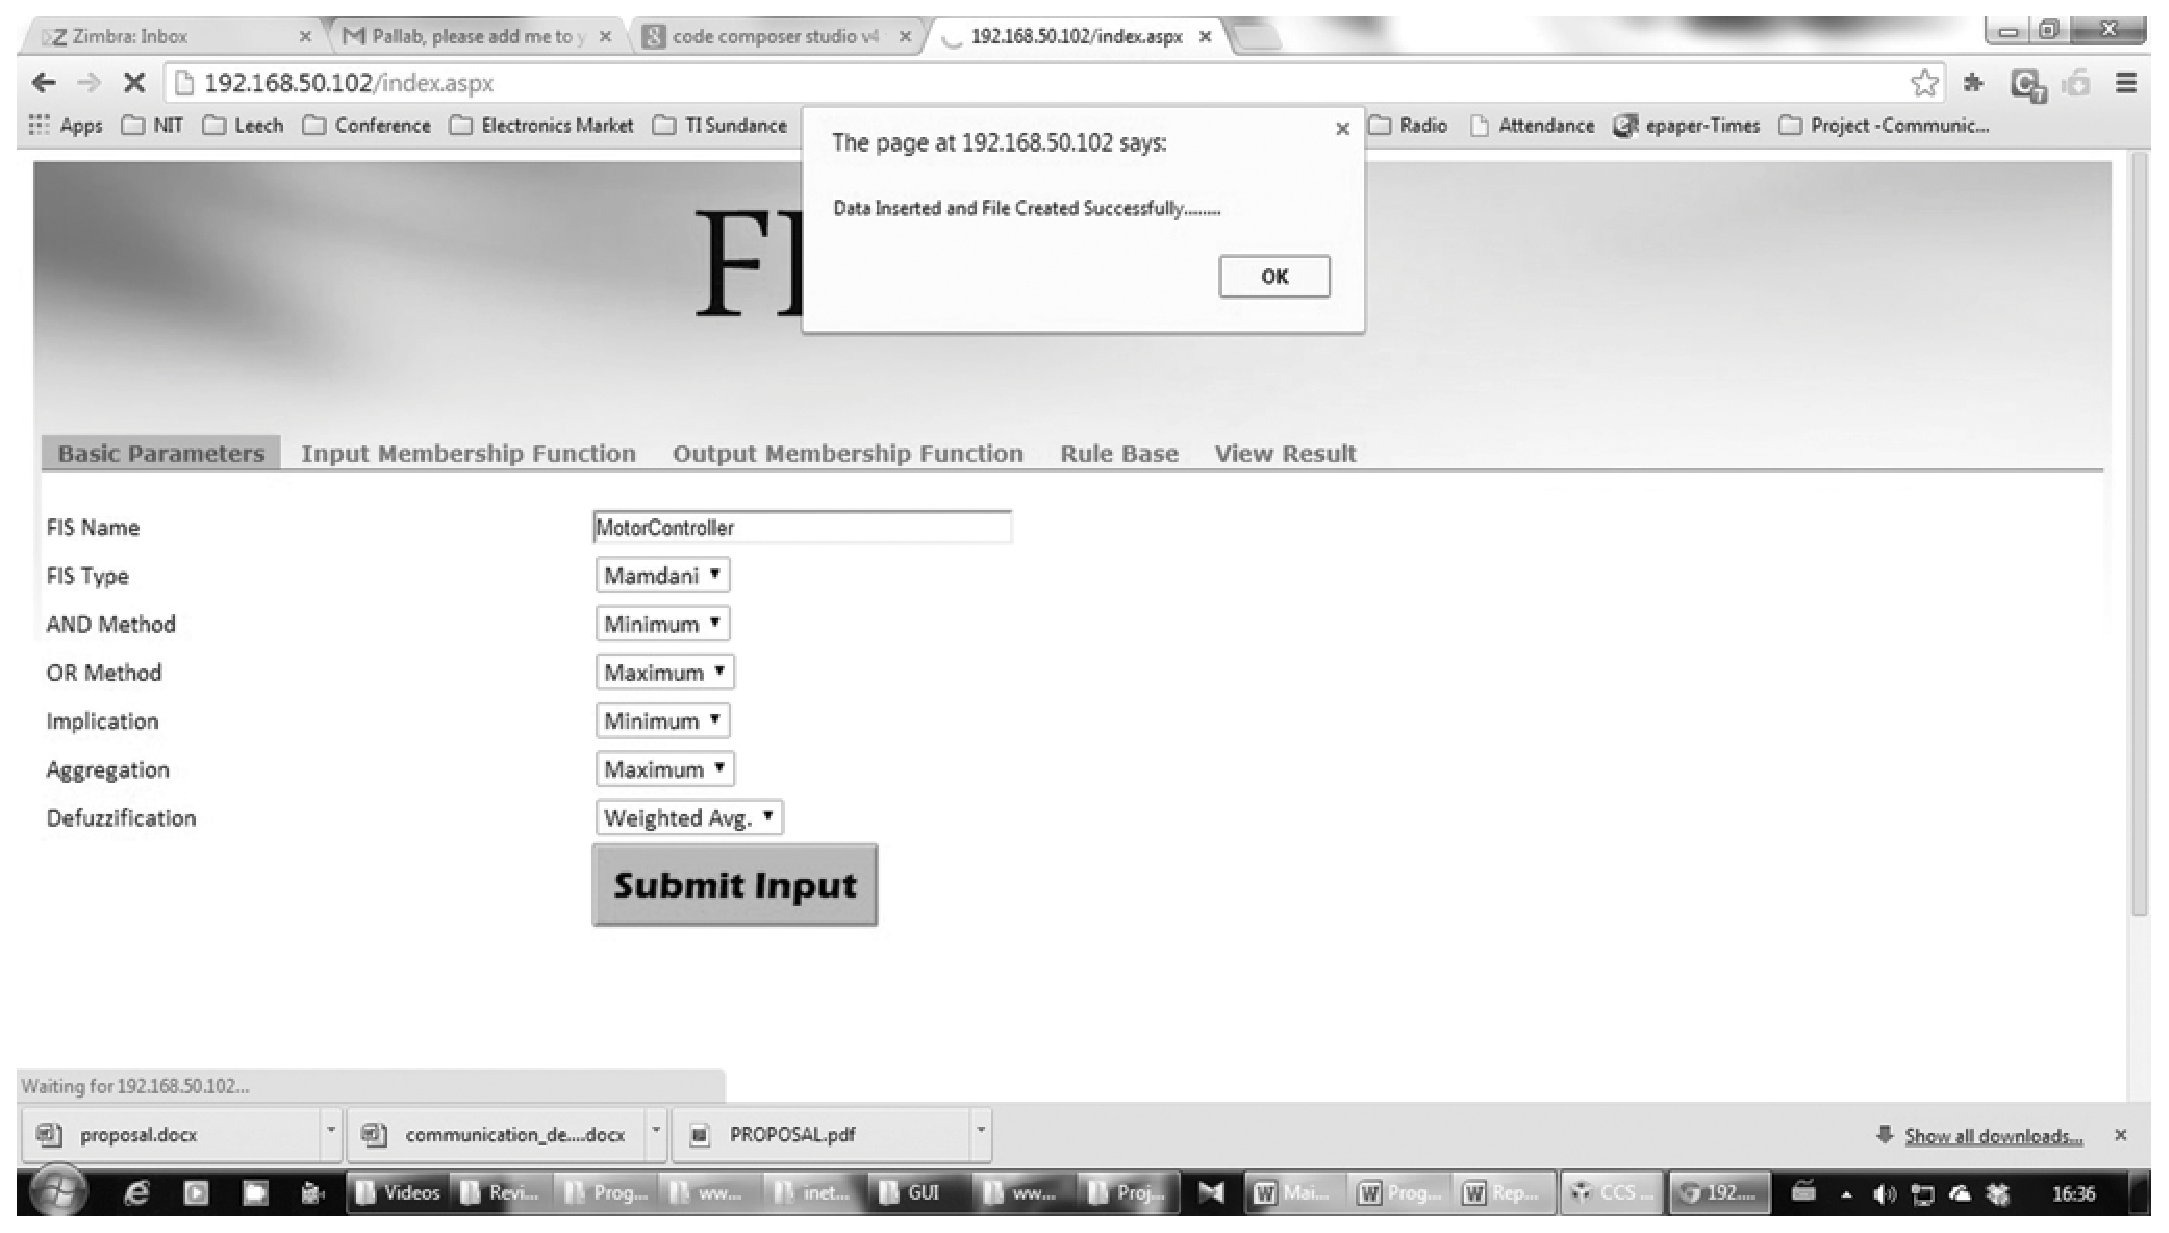
\includegraphics[width=1\linewidth,height=12cm]{Chapter4/chapter4/Fig3.eps}
	\caption{Simulink Model for Speed Control of DC Motor}
	\label{fig:SimulinkModelforSpeedControlofDCMotor}
\end{figure}

A Simulink model to simulate Speed Control of a DC Motor with PID and Fuzzy Logic Controllers is tested in this experiment \cite{malla2012,twotank2012}. The Simulink model of the process plant is presented in Figure \ref{fig:SimulinkModelforSpeedControlofDCMotor}. The control problem uses a DC Motor with Armature Resistance $ (R_A) $ = 1 $\Omega $, Armature Inductance $ (L_A) $ = 0.5, Inertia $ (J_M) $ = 0.01, Damping $ (B_M) $ = 0.1, Torque Constant $ (K_{\tau}) $  0.01 Nm/A and Back EMF Constant $ (K_B) $ = 0.01 Vs/rad. Transfer function of the plant model is stated as:
\begin{align} \label{eq:1}
\frac{\theta {\rm (}s{\rm )}}{V_A{\rm (}s{\rm )}}{\rm =\ } \frac{K_{\tau }}{L_AJ_Ms^{{\rm 3}}{\rm +}\left(R_AJ_M{\rm +}L_AB_M\right)s^{{\rm 2}}} \nonumber\\
{\rm x\ } \frac{1}{\left(K_{\tau }K_B{\rm +}R_AB_M\right)s}
\end{align}

The ACDC Motor is controlled by FLC and PID controllers in different datapaths. Simulation of this model produces the I/O dataset and is saved in a file which concludes first phase of this experiment. The data set consists of two inputs, error in speed and its derivative, and the control signal (voltage to the DC Motor) as an output.

\subsection{Hardware-in-Loop Test} \label{sec:hil}
The Hardware-in-the-Loop (HIL) testing method is a prevailing testing method in industries. It has been exploited to test wide array of embedded system applications over past two decades. It was initially introduced in the Aviation industry. The major factor which makes this test methodology prevalent in the industry over the years are time to market and its low complexity. HIL test method caters an efficient platform to test real-time system designs by adding the plant complexity to be controlled in the test platform. The plant model and all related dynamic systems under control is mathematically presented. This algebraic representation of the entire plant model is called as the ``plant simulation''. The real-time embedded system is tested by interacting with this plant simulation which executes in a computer, sometimes referred to as the Host Computer. Figure \ref{fig:HIL} shows the main concept of the HIL test methodology where an embedded system is developed on a real-time processor and is interacted with the process plant simulation in the host computer.

\begin{figure}[h!]
\centering

\includegraphics[width=0.9\linewidth]{Chapter4/chapter4/HIL}
\caption{Test Setup for Hardware-in-Loop Testing of G-FLCS}
\label{fig:HIL}
\end{figure}

The proposed MT-FRHC based G-FLCS is developed on a TI C6748 DSP processor. This represents the embedded system under test in the HIL loop. The dynamic modeling of the ACDC Motor is developed in Simulink. This represents the ``plant simulation''. The HIL test was performed as depicted in Figure \ref{fig:HIL}. From executing the ``plant simulation'' with controllers developed in Simulink provides the simulated results. Figure \ref{fig:SimulinkModelforSpeedControlofDCMotor} represents the ``plant simulation'' model. This model is developed based on the transfer function derived in \eqref{eq:1}. The results from simulation and HIL test was compared and analyzed where an error of 2\% was recorded. Details of this test in provided in section \ref{sec:perfanal}. However, before analyzing the performance, a method for FCP generation is explained in section \ref{sec:fcpgen}. This method was found to decrease the time consumed by GA based FCP extraction at large.  

\begin{figure}[h!]
	\centering
	\subfloat[Simulation output for the Armature Controlled DC Motor]{\label{fig:SimulationoutputfortheArmatureControlledDCMotor}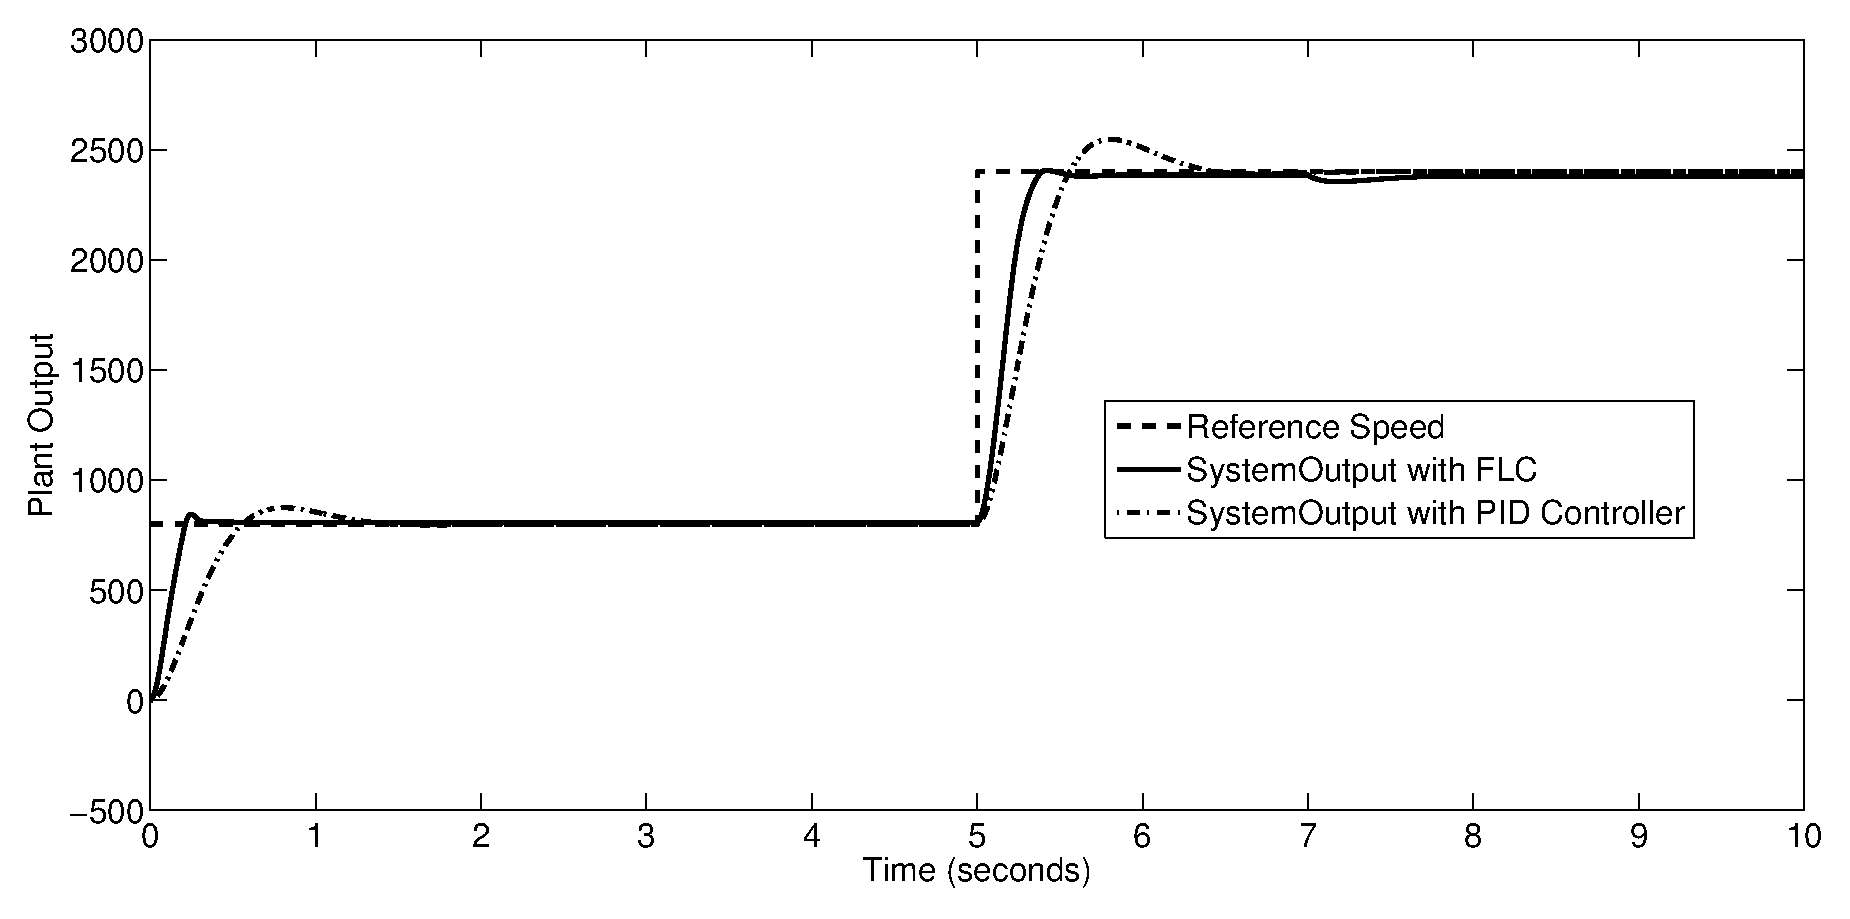
\includegraphics[width=0.95\linewidth]{Chapter4/chapter4/Fig4.eps}} \\
	\subfloat[Control Signal Data plot for Simulated and hardware G\hyp{}FLCS]{\label{fig:ControlSignalDataplotforSimulatedandHardwareFLC}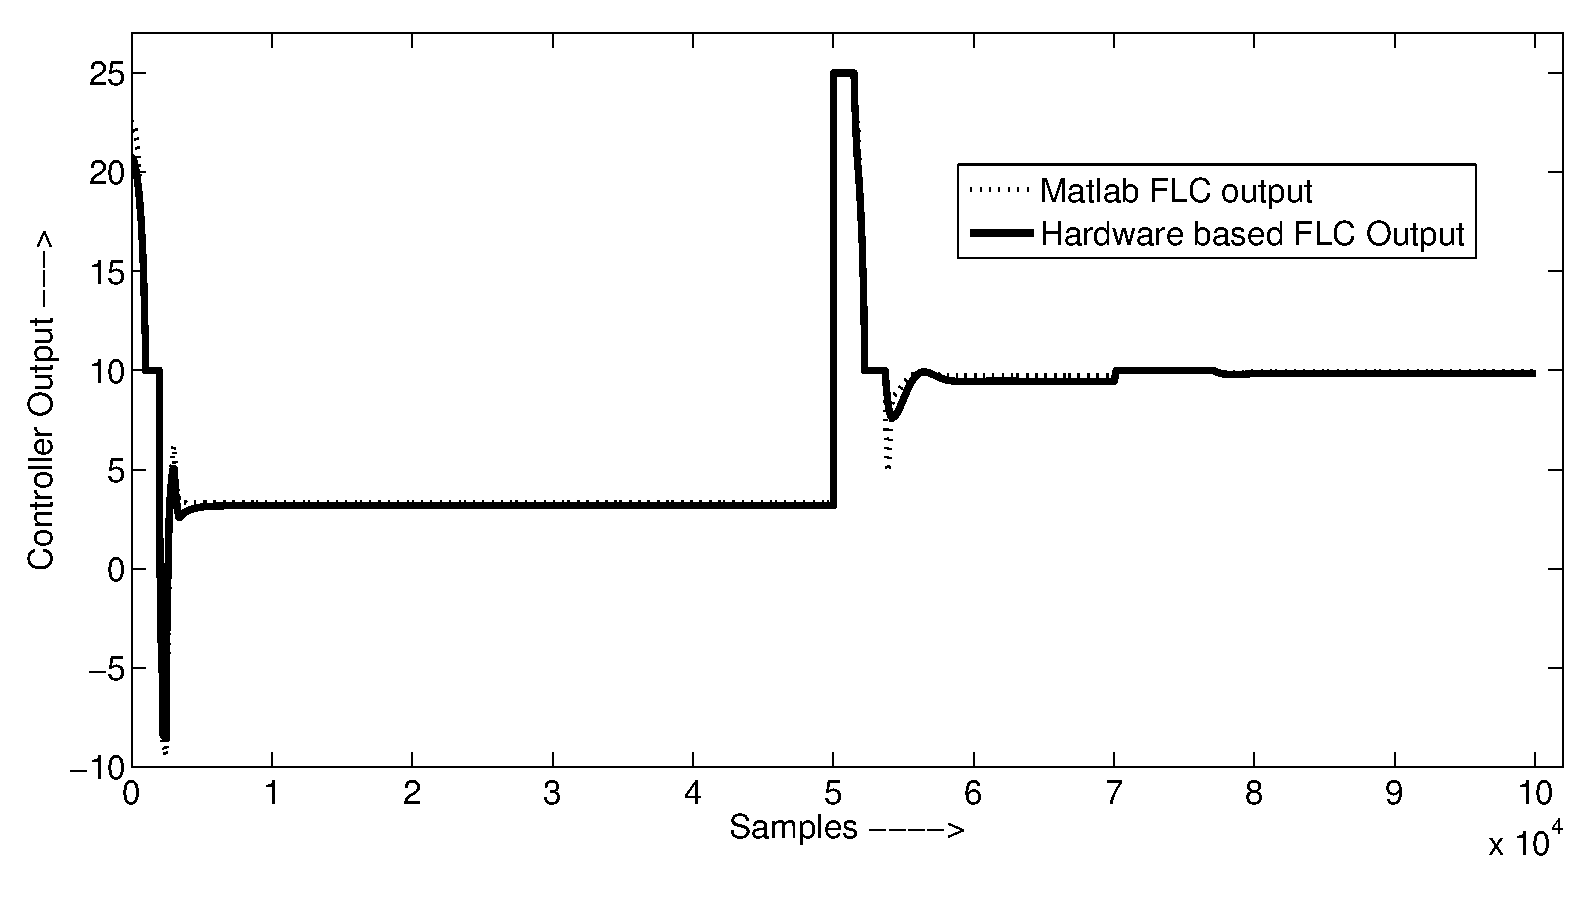
\includegraphics[width=0.95\linewidth]{Chapter4/chapter4/Fig5.eps}}
	\caption{Plant output and Controller output of ACDC Motor simulated using Matlab Fuzzy Logic Toolbox and HIL test with proposed hardware G\hyp{}FLCS} 
	\label{fig:SimulationOut}
\end{figure}

\subsection{Fuzzy Control Parameter Generation} \label{sec:fcpgen}
A genetic algorithm based fuzzy control parameter extraction technique is described in section \ref{sec:FCP}. However, in many of the test processes, it is found the genetic algorithm based FCP extraction technique extensively time consuming. One way of reducing this extraction time is by providing initial parameters to the GA. With proper initial parameters the search space for GA can decrease drastically. This can reduce the FCP extraction time. One of the widely used techniques for FLCS design is a Fuzzy approximation of PID controller \cite{Lin2009,Wang1992a}. The FCP generated from this scheme assume a FLCS structure analogous to classical PID controller \cite{Murray2009,bookBehera2009,Arun2014,bookBogdan2006a}. However unlike classical PI controller, Fuzzy PI controller is non\hyp{}linear. This method implicitly implies that the generated FCP will consistsof fuzzyinput fuzzy variable $ e $ and $\Delta e$. The FCP used for this Initial parameters for GA based FCP is finallys \cite{Sahu2015,Demir2011b}. The FCP used for this G\hyp{}FLC syst system for verification of the controller\footnote{File can be downloaded from \url{https://goo.gl/83bVna}}. 

In algorithm \ref{algo:1}, a plant simulation model with PID controller is developed on Simulink as described in section \ref{sec:hil}. An input-output relationship between the error signals (consisting of $ e $ and $\Delta e$) and control output ($ u $) is generated and recorded for large number of samples. Introduce input MF corresponding to maximum and minimum values of inputs $ e $ and $\Delta e$. Similarly, for each set of input membership functions introduced, a corresponding MF is introduced. The kernel of these MFs are set to the respective minimum and maximum output value from the dataset. In this algorithm, initial choice of the memberships are trapezoidal and for every other iteration, triangular membership functions are added appropriately.     

\begin{algorithm}[h!]
	\caption{A technique for Fuzzy PI Approximation}\label{algo:1}
	\begin{algorithmic}
		\Procedure{Error and Control Signal Generation}{}
		$\textit{N} \gets \text{Mamimum no. of membership functions allowed}$
		\State \emph{top}:
		\State $i = i + 1$
		\State Run Simulink Model with PID Controller
		\State $\textit{e}, \Delta e \gets \text{Error signal at each sample}$
		\State $u \gets \textit{Control signal generated at each sample}$
		\State Note \textit{u} at maximum and minimum value of \textit{e} and $\Delta e$
		\State \emph{loop}:
		\State Introduce input MF corresponding to minimum and maximum value of \textit{e} and $\Delta e$
		\State Introduce output MF corresponding to minimum and maximum value of \textit{u}
		\State Addition of triangular MFs to map rules as introduced above
		\State Evaluate rules at minimum and maximum \textit{e} to generate $\hat{u}$ 
		\State
		\eIf {$i < N$}{
			\eIf {$u-\hat{u}\neq0$}
			{\State \textbf{goto} \emph{loop}.}
			{\State \textbf{goto} \emph{top}.}
		}
		{
			\State \textbf{close}; 
		}
		\EndProcedure
	\end{algorithmic}
\end{algorithm}

\subsection{Performance Analysis} \label{sec:perfanal}
\begin{table}[b!]
	\centering
	\caption{Results from hardware G\hyp{}FLCS experiment with Simulink Model}
	\label{tab:Results}
	\begin{tabular}{ll}
		\hline
		\noalign{\vskip 2mm} 
		Output Parameters & Observation \\ \hline
		\noalign{\vskip 2mm} 
		Total data Samples & 100021 \\
		Total Execution Time & 7.248989 s \\
		Average Execution Time & 7.247427e-005 s \\
		FLIPS & 13.8 K \\
		Percentage Error & 2\% w.r.t. Matlab FIS \\
		Mean Square Error (MSE) & 0.1298 \\ \hline
		\noalign{\vskip 2mm} 
	\end{tabular}
\end{table}	

A HIL test was conducted for the proposed MT-FRHC based G-FLCS on TI C6478 as described in section \ref{sec:hil} for the plant model shown in Figure \ref{fig:SimulinkModelforSpeedControlofDCMotor}. The response of the HIL test was recorded and tabulated in Table \ref{tab:Results}. The controller performance has been analyzed with respect to inference time and control output separately and plotted in Figure \ref{fig:SimulationOut}. The simulation experiment was found to work seamlessly. The hardware realization of the proposed G-FLCS application was necessary to determine if this approach is perceivable in real\hyp{}time.

\subsubsection{Performance Analysis: Control Output} \label{sec:ContPerf}

The output from HIL test is conducted for the Simulink model in Figure \ref{fig:SimulinkModelforSpeedControlofDCMotor} and the output presented in Figure \ref{fig:SimulationoutputfortheArmatureControlledDCMotor}. The inputs and corresponding output was recorded and saved in file which is intended to be used as data source. The same FCP file used in this simulation was loaded in the FLC based DSP hardware through the server application as described in chapter 3. A separate Windows application was created to read the input data stored in the data source file and send to the G\hyp{}FLCS externally. 
\par		
The G\hyp{}FLCS received the inputs and generated suitable control outputs which was sent back to the PC and recorded in a loop. The recorded data is then compared to actual simulated output for data validation. The time elapsed in this entire process has also been recorded. The inferences observed during this experiment has been tabulated in Table \ref{tab:Results}.
There were total of 100021 input samples in this entire simulation. Control signals generated from the simulation and G\hyp{}FLCS was recorded for each input samples and plotted in Figure \ref{fig:ControlSignalDataplotforSimulatedandHardwareFLC}. This figure represents a plot of the control output corresponding to the DSP based proposed G-FLCS and Matlab FLT for all the input samples. It validates that the control data output from the G\hyp{}FLCS is in synchronization with the simulated result with a MSE of 2\%. There is a slight deviation observed in control output of the G\hyp{}FLCS and Simulink simulation. This can be attributed to the design and implementation of MT-FRHC rule reduction technique with VBCoA defuzzification method as discussed in chapter 2. 

\subsubsection{Performance Analysis: Inference Time}
\par
The system has also been tested for its inference time. Inference time is defined as the time taken for a set of input to propagate to the output and produce a control action. Figure \ref{fig:ControlSignalDataplotforSimulatedandHardwareFLC} provides no observation related to the execution time of the G\hyp{}FLCS. Thereby, time elapsed in the entire process of testing with 100021 samples was also been recorded. It found to be 7.248949 seconds for entire process and on average 0.073 ms or 73 $\mu$s for single inference. This data provides an estimate of the inference time that can be achieved with the proposed G\hyp{}FLCS. However it is should to be noted that this time does not include any instance where parameters have tuned in between the process. 

\subsection{Comparison to Existing Works}
The G\hyp{}FLCS design is implemented on a programmable DSP. There are few works reported in the literature which implements similar designs on FPGA platform. However, these systems provide fewer flexible FCP features in comparison to the proposed design. The performance of the proposed G-FLCS was compared to the existing FPGA based designs presented in \cite{Millan2008,Fu2010}. A summary of these designs are tabulated in Table \ref{tab:feature}. It can be observed that the proposed G-FLCS design provides variety of features with adequate speed and flexibility in comparison to the FLCS designs reported in \cite{Millan2008,Fu2010}. This design provides a speed of approximately 13 KFLIPS for a 2\hyp{}input 1\hyp{}output system with 49 rules with seven MFs for each input and output. The proposed G\hyp{}FLCS is designed to support a maximum 4\hyp{}input 1\hyp{}output system with seven MFs for each input and output space. This adds up to a total of 2401 rule system. The code size of 61 \% reported in Figure \ref{fig:Mem_Util} implements 4-input 1-output system. 

\begin{table}[h!]
	\centering
	\caption{Comparison between Proposed hardware G\hyp{}FLCS and Similar Designs based of Reconfigurable Parameters}
	\label{tab:feature}
	\begin{tabular}{lllll}
		\hline
		Year & Reference & Speed & Platform & Features \\ 
		&  & (in FLIPS) &  &  \\ \hline
		2008 & Millan et. al.\cite{Millan2008} & 5.5 K & FPGA & \begin{tabular}[c]{@{}l@{}}Output MFs: Singleton (5)\\ I/O: 2-1\\ Input MFs: 8\\ Overlaps: Dynamic\\ Rules Evaluated : 64\end{tabular} \\ \hline
		2010 & Yi Fu et. al.\cite{Fu2010} & 11 K & FPGA & \begin{tabular}[c]{@{}l@{}}Output MFs: (5)\\ I/O: 2-1\\ Input MFs: 5\\ Overlaps: 2\\ Rules Evaluated : 25\end{tabular} \\ \hline
		\multicolumn{2}{l}{Proposed G-FLCS} & 13 K & DSP &  \begin{tabular}[c]{@{}l@{}}Output MFs: (7)\\ I/O: 4-1 (Configurable)\\ Input MFs: 7\\ Overlaps: Dynamic\\ (4)\\ Rules Evaluated : 49\\ (2401)\end{tabular} \\ \hline
	\end{tabular}
\end{table} 


\section{Summary}
The realization of the remotely tunable MT-FRHC based G-FLCS with VBCoA defuzzification on programmable DSP hardware is explained in this chapter. This technology opens line of approach for implementation to several explorations. The motivation behind this research was deployment of a generic fuzzy framework with complex features in a programmable device such that it can be remotely tuned by altering its parameters in real\hyp{}time. In this chapter, a successful implementation of these objectives is described. Existing G-FLCS have been able to produce significant speed by reducing functionalities in their architecture. This architecture provides large number of functionalities to its users along with sufficient speed to drive most industrial processes. This system is standardized with MATLAB Fuzzy Logic Toolbox and has ability to incorporate FIS files generated by this toolbox. This system presents a framework for remotely tunable MT-FRHC based G-FLCS that can suitably replace other controllers by following the design protocols explained in this thesis. The proposed systems is observed to perform well within the multiple testing paradigms. Through investigations have been done using multiple applications to ascertain its generality and applicability. In summary, this chapter successfully presents a remotely tunable MT-FRHC based G-FLCS with VBCoA module developed on programmable DSP with interface to a WebUI which can operate as standalone controller with an operating speed of around 13K FLIPS.

